% ------------------------------------------------------------------------------
% A primer on continuum models and how this relates to the work we have done
% 1) Introduce logistic growth and diffusion
% 2) Introduce FKPP in all its glory .
% 3) Show one and two d spread
% 4) Couple to the sub-grid, what this says about the sub-grid...
% 5) Talk about growth rate-xi and growth rate of sub-grid... an assumption about mixing and SIR <--         appendix territory
% 6) Show `toy model properties in xi and d' get realistic looking spread...
% 7) Show realistic spread and give a primer to things which could be done.
% 8) Talk about alternate more, non-linear models and consult Rammile...
% ------------------------------------------------------------------------------

\chapter{Towards landscape-level control}

% In reality, connectivity between patches depend on the dispersal kernel, and not on an arbitrarily defined nearest-neighbour structuring element.
% Connectivity between patches can extend radially non-locally over a number of surrounding patches.

\label{ch7:landscape-level-control}

In this final science Chapter, we will examine how host heterogeneity, under the influence of a wind-dispersed pathogen, 
can give rise to natural pinch-points and fault lines in the spatial distribution of hosts in Great Britain. 
Population pinch points may give rise to a bottleneck in the epidemic spread, which in principle could be exploited with targeted epidemic control to fragment the host population with minimised effort. 
In essence, a strategy of 'regional containment', targeting the local wind-based pathogen dispersal mechanism, 
is formulated and scaled up over Great Britain.
Similar concepts for crop and livestock diseases have been articulated \cite{PAPAIX201435, GILIOLI20131, Gilligan-disease-management}, yet to our knowledge, this has not been examined rigorously nor generalised to tree populations over large spatial scales.

A great deal of research has been carried out to understand the optimisation of control in crop and tree-based epidemics\textemdash as reviewed in section \ref{ch2:lit-rev-compartmentalised-models}. 
Spatial structure is an essential factor when considering how to manage an outbreak \cite{spatial-control-optimisation, control-heterogeneous-landscapes}. 
The mainstream paradigm of control typically considers infected tree removals over a relatively small spatial scale, near infected hosts \cite{WEBIDEMICS}, or, more broadly, ahead of the wavefront \cite{large-scale-control}. 
However, landscape-level epidemic control, based solely on the structure of large-scale spatial distribution of hosts incorporating topography, has yet to be explored in-depth.

Section \ref{sec:fragmentation-method} presents a novel method to disrupt epidemic connectivity in the host distribution.
Following on, the method is analysed in section \ref{sec:towards-regional-control}. However, the analysis constitutes unfinished work and sets the scene for future research questions.
The work conducted in this Chapter rests on the $SEIR$ model of ADB, although the outlook is less specific to ADB and more general-purpose, suitable to any class of wind-dispersed tree pathogens with comparable dispersal parameters. 


% - The challenge of controlling ADB reflects the challenge of containing a pathogen that spreads via long-distance dispersal (LDD). 
% Moreover, HP can infect ash through diverse mechanisms such as water-course and contaminated soil and LDD means that new and distant foci can emerge over large distances without the need for nearby ash\textemdash for a more detailed review of ADB, including the challenges of control and biology, see chapter \ref{chapter2:litrevieiw}.
% Subsequently, we found connectedness inside a given cluster could depend on just a small number of `connecting points' which if removed, thinned below $\rho_c$, would lead to significant fragmentation and divide the cluster

% - This leads us to develop a heuristically-based fragmentation algorithm
% - In section X map connectivity will be examined under a threshold function \Phi(\xi). 
% -As we define it, fragmentation considers which locations in the population, if artificially taken below $R_0 = 1$ through felling, would disrupt epidemiological connectivity\textemdash, thus leading to containment. 
% -Epidemic containment in the largest $R_0$-cluster is then analysed and shown to be most applicable over a specific range of infectivity parameters.
% -Although the strategy of control presented in this chapter is demonstrated on a simplified model of ADB, the results are generic and could be applied to any wind-dispersed pathogen.
% - Developing a landscape-level control strategy when there is LDD (and epidemic uncertainty) present several obstacles, 
% - The emergent epidemic caused by the pathosystem ash dieback (ADB) is predicted to wipe out the vast majority of ash in Great Britain over the next few decades \cite{ash-dieback-costs}. 
% - Currently, large-scale control efforts aim to slow the spread, in contrast, to complete containment. % Find references of current efforts/guidelines 
% - A slower rate of spread benefits ash populations allowing them to recover alongside artificial replanting. % reference 


% Classical percolation theory requires lattice points to be independently open or closed, with no dependence on the state of nearest neighbours. So, strictly speaking, the analogy to percolation breaks down because the susceptibility of a given patch of ash is likely dependent on its neighbours $R_0$-value; as can be seen in Figures \ref{fig:uk-mapping}(d-e), particularly in the south of England where ash densities are high. 
% Heterogeneity in the $R_0$-map becomes particularly useful in the the next chapter, where we investigate a potential strategy of landscape-level control based on disrupting epidemic connectivity and fragmentation.
% Before we can move towards epidemic control, it is desirable to understand $R_0$-clustering more fully.
%-----------------------------------
% Assuming connectivity
% Patches below the threshold present a natural barrier to ADB spore dispersal between clusters, for two reasons: 
% 1) Below-threshold patches do not support high levels of infected biomass, spore dispersal emanating from these patches will therefore be lessened.
% 2) The domain resolution, configured in section \ref{ch6:re-scaling-host-data}, ensures that no secondary infections will result for the parameter values and spatial scale under consideration in the seasonal $SEIR$ model of ADB.
% Likewise, 

\section{Method: cluster fragmentation}
\label{sec:fragmentation-method}

In Chapter \ref{ch:6-adb}, $R_0$-clusters were introduced.
Clusters of susceptible patches of land in the $R_0$-map revealed which regions in Great Britain are likely to be the most severely devastated by the pathogen. 
Whereas patches below the threshold present a natural barrier to the spread of disease;
in this simplified interpretation, below-threshold patches can be presumed to not support high levels of infected biomass and infectious spore production.
Moving forward, we assume that the pathogen will remain confined within isolated $R_0$-clusters and not spread through patches below $R_0=1$.
Undoubtedly, several assumptions underpin this argument, including the omission of LDD, both wind-borne and human-mediated, alongside stochastic outbreaks below the threshold.
 
Here, epidemics propagating through the $R_0$-map describe a `\textit{percolation-like}' problem, with the caveat of clustering.
If no control is attempted, all patches within a susceptible cluster are put at risk if one patch becomes infected; 
this motivates a control strategy based on cluster fragmentation to accomplish regional containment.
Specifically, by artificially reducing $R_0$ in a small number of identified patches, connectivity within the cluster can be efficiently disrupted with minimal effort.
Cluster fragments then define disconnected `sub-clusters' (e.g. $\mathbf{C_1}$ and $\mathbf{C_2}$) that eliminates risk for trees inside one sub-cluster.
Host patches inside the confining cluster are assumed to be removed (or put at risk) by the pathogen, while hosts inside the remaining sub-cluster are saved and remain susceptible.
Efficient control is achieved if the control effort is small compared to the reduction of epidemic impact.

% - The modelled distribution of ash depicts a continuum of connectivity throughout Great Britain.
% - The shape of each cluster is constrained by landscape topography and geography. 
\subsection{Identifying high-priority patches}
\label{sec:fragmentation-method-1}

An algorithm was developed to identify high-priority patches in the host distribution, which disrupts epidemic connectivity if taken below the threshold.
Given a CCA-identified cluster in the $R_0$-map, $\mathbf{C}$, we can define a binary-valued threshold function $\Phi(\xi)$ by:
\begin{align}
\label{eq:xi-step}
\Phi(\xi) = \left\{ \begin{array}{cc} 
                1 & R_0(i, j) \geq \xi \\
                0 & R_0(i, j) < \xi \\
                \end{array} \right.
\end{align}

where $R(i,j)$ is the patch-level reproduction ratio at spatial coordinates $(i,j)$ in $\mathbf{C}$.
The parameter $\xi$ takes values in interval $\big[1, \mathrm{max}\big( R_0(i,j)\big) \big]$, 
where $\mathrm{max}\big(R_0(i, j)\big)$ is the highest value of $R_0$ in $\mathbf{C}$\textemdash henceforth denoted by $R_{max}$.

\begin{figure}
    \centering
    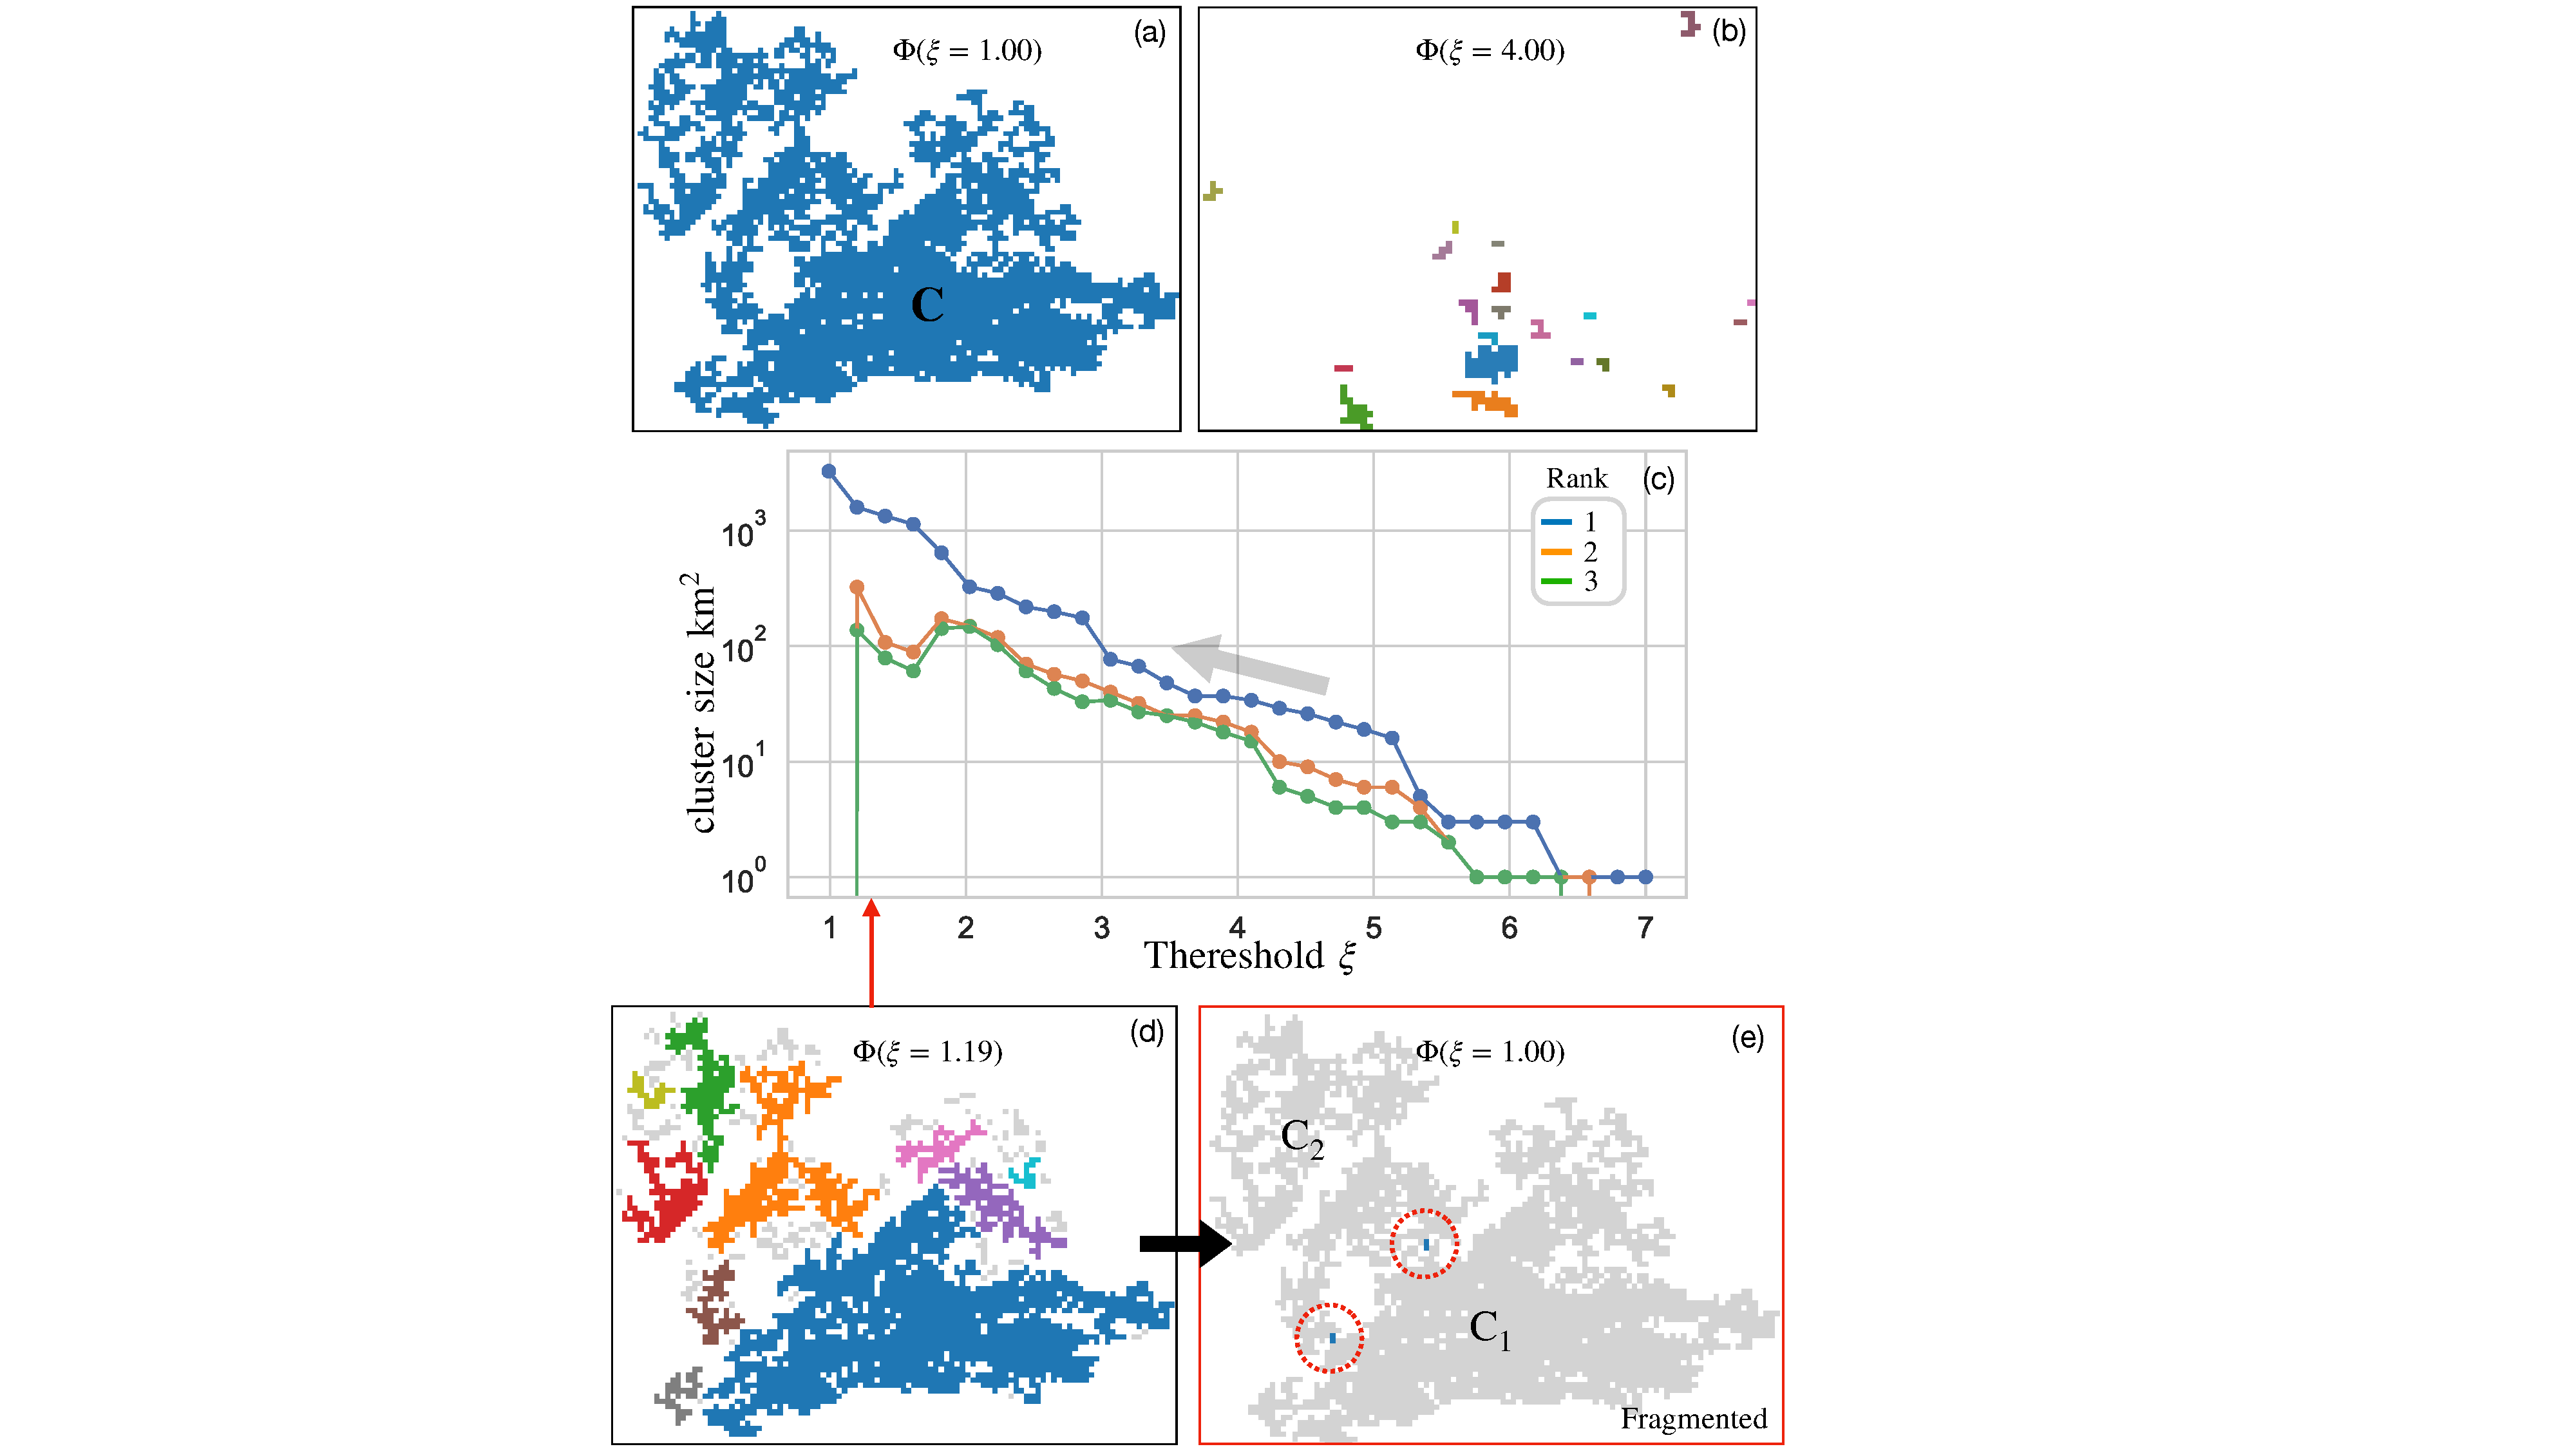
\includegraphics[scale=0.5]{chapter7/figures/figure1-frag-method.pdf}
    \caption{
    A graphical illustration of the algorithm developed to fragment $R_0$-clusters.  
    (a) The largest cluster, denoted by $\mathbf{C}$, is shown inside an arbitrary domain at resolution $3\mathrm{km} \times 3 \mathrm{km}$ and infectiviy $\beta^*=450$ for the model $\phi_1$-ga.
    Applying the threshold function $\Phi$ at $\xi=1$ recovers the $\mathbf{C}$ exactly because all patches are above the threshold $R_0=1$.
    (b) Applying the threshold function $\Phi$ at $\xi=4$ yields a low-density map with sparsely distributed clusters, as few patches surpass $R_0\geq 4$. 
    (c) The top three largest clusters, by area $\mathrm{km^2}$, are shown as a function of $\xi$.
    (d) At specific values of $\xi$, some sub-clusters join to form larger clusters\textemdash here, the blue and orange clusters proceed to join at $\xi = 1.15$.
    (e) Connecting patches are identified when large discontinuities arise when back-stepping $\xi \rightarrow \xi -\delta \xi$, shown here by the blue pixels; removing these patches fragment the cluster $\mathbf{C}$ in $\mathbf{C_1}$ and $\mathbf{C_2}$. 
    }
    \label{fig:R0-threshold-function}
\end{figure}

Figure \ref{fig:R0-threshold-function} shows how the function $\Phi(\xi)$ allows the identification of high priority spatial locations.
In Figure \ref{fig:R0-threshold-function}(a) we begin with a target-cluster, $\mathbf{C}$, shown in blue;
$\mathbf{C}$ is the largest cluster detected in an arbitrary $R_0$-map for the model $\phi_1$-ga and infectivity $\beta^*=450$ (as described previously in Chapter \ref{ch:6-adb}).
Applying the threshold function $\Phi(\xi=1)$ recovers $\mathbf{C}$ entirely, as all patches in $\mathbf{C}$ are over the threshold.
In contrast, larger values of $\xi$ result in a lower-density map with sparsely distributed clusters, 
demonstrated by the small number of labelled clusters in Figure \ref{fig:R0-threshold-function}(b) at $\Phi(\xi=4)$.
Similarly, only one (or at most a handful) of patches populate the domain at the limiting value $\Phi(\xi=R_{max})$.

Connected component analysis (CCA) is performed at each step $\xi \in [1, R_{max}]$ in order to identify and label sub-clusters. 
At particular steps $\xi \rightarrow \xi - \delta\xi$ (i.e. back-stepping), $\mathbf{C}$ will begin to form when distinct sub-clusters\footnote{
It is possible that three or more sub-clusters suddenly connect to form $\mathbf{C}$ in the same step; 
these complexities are taken into account by the algorithm.} 
 (e.g. $\mathbf{C_1}$ and $\mathbf{C_2}$) suddenly connect when certain critical links become non-zero\textemdash
analogous to the formation of a spanning cluster opening up in a percolation. 
Figure \ref{fig:R0-threshold-function}(d) depicts a scenario with a number of disconnected sub-clusters at $\xi=1.19$ that merge together at $\xi=1.15$.
The `binary dilation' operator \cite{liang1989erosion, 23111, nachtegael2001connections} was used to detect all the patches which become non-zero and bridge sub-clusters, as elaborated in Appendix \ref{sec:a-binary-dialator}.
Henceforth, `connecting patches' refer to patches that connect sub-clusters in a discontinuity step.

When $\mathbf{C_1}$ and $\mathbf{C_2}$ abruptly merge to form the basis of $\mathbf{C}$, a significant discontinuous jump in cluster size is detected. 
All spatial locations $(i,j)$ which bridge the gap between $\mathbf{C_1}$ and $\mathbf{C_2}$ are then identified and removed by taking $R_0$ below the threshold.
Figure \ref{fig:R0-threshold-function}(e) shows two singular patches in blue (and highlighted in red) that if taken below $R_0=1$,
would fragment $\mathbf{C}$ into two sub-clusters $\mathbf{C_1}$ and $\mathbf{C_2}$.
Successive steps through $\xi$ continue until $\xi=1$.
For each discontinuity event, connecting patches are detected and removed from the system,
thus preventing $\mathbf{C_1}$ and $\mathbf{C_2}$ from merging over $\xi \in [1, R_{max}]$.
In this manner, the target-cluster $\mathbf{C}$ is fragmented into two separate sub-clusters. 
As we can see, connectedness within the domain can depend on a small number of patches.

\subsection{Iterative cluster fragmentation}
\label{sec:fragmentation-method-2}

Each $R_0$-cluster can be iteratively fragmented $N$ times to produce a set of disconnected sub-clusters, 
where, on average, each fragmentation iteration produces $N+1$ sub-divided clusters.
Figure \ref{fig:iterative-fragmentations} demonstrates the iterative process for the example cluster $\mathbf{C}$ from Figure \ref{fig:R0-threshold-function}(a).
During first iteration the target cluster $\mathbf{C}$ is fragmented into $\mathbf{C_1}$ and $\mathbf{C_2}$, shown respectively in Figure \ref{fig:iterative-fragmentations}(a) as orange and blue.
After each iteration, sub-clusters are ranked according to the area they cover, the next iteration proceeds by targeting the largest sub-cluster;
this is illustrated in Figure \ref{fig:iterative-fragmentations}(b) when $\mathbf{C_1}$ is targeted during the next iteration at $N=2$, producing a third disconnected sub-cluster ($\mathbf{C_3}$) shown in green. 
The process is then repeated $N=10$ times to produce $11$ disconnected fragments in Figure \ref{fig:iterative-fragmentations}(c).

\begin{figure}
    \centering
    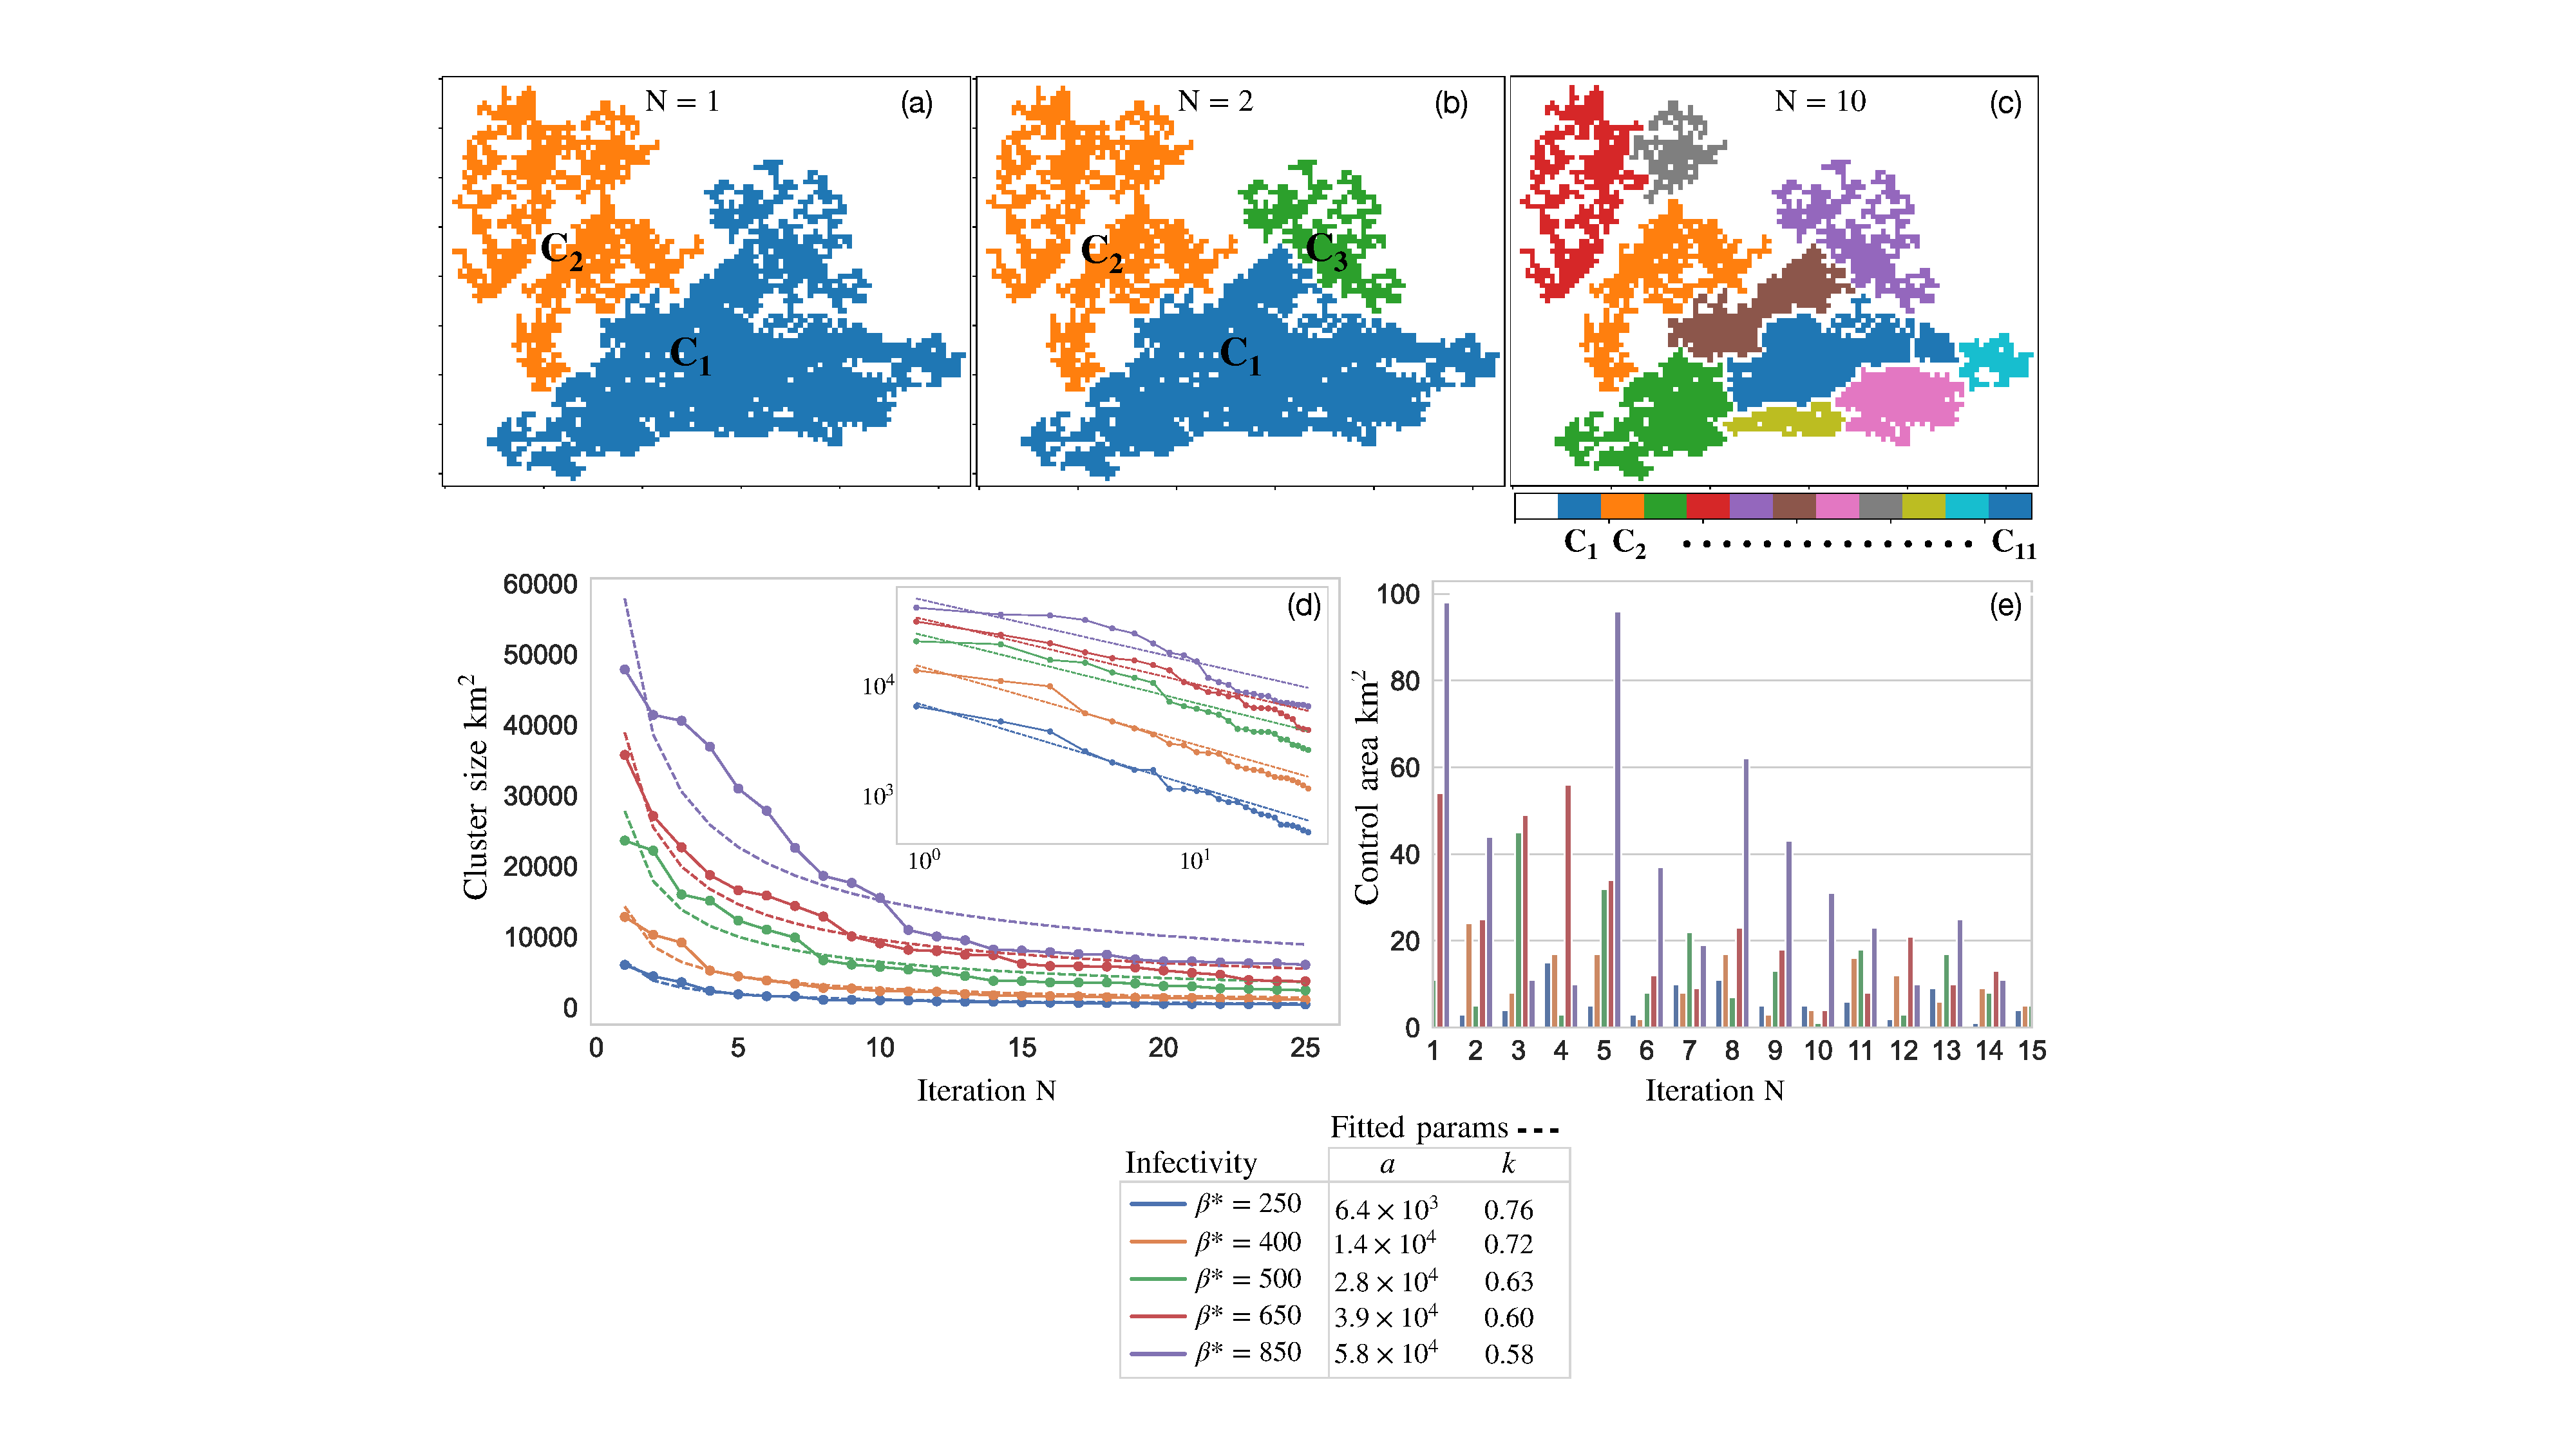
\includegraphics[scale=0.41]{chapter7/figures/figure2-Iiterative-frag.pdf}
    \caption{
    The fragmentation algorithm is shown as an iterative process. 
    (a) The example cluster ($\mathbf{C}$) is fragmented into two sub-clusters ($\mathbf{C_1}$ and $\mathbf{C_2}$) during the first iteration of the algorithm.
    (b) During the next iteration, the largest sub-cluster $\mathbf{C_1}$ is targeted to produce an additional cluster fragment, denoted here by $\mathbf{C_3}$ in green.
    (c) The process is iteratively repeated $N=10$ times to produce $11$ sub-dived clusters.
    (d) The sub-cluster size reductions are plotted for $25$ iterations of the algorithm over a range of infectivity parameters;  
    approximately, size-reduction follows an inverse power law, as indicated by the corresponding fitted dashed lines.
    Lower infectivity parameters correlate to an efficient fragmentation in contrast to higher $\beta^*$ values\textemdash suggested by the logarithmic inset plot.
    (e) The area of connecting patches, or `control area', is plotted against the iteration\textemdash truncated to $15$. 
    Generally, the number of connecting patches increases with infectivity and decrease with iteration.
    }
    \label{fig:iterative-fragmentations}
\end{figure}

Figure \ref{fig:iterative-fragmentations}(d) shows the sub-cluster size reductions for $N=25$ iterations and a number of different infectivity parameters.
For all infectivity parameters considered, the largest sub-cluster continually decreased for each iteration of fragmentation.
Moreover, cluster size reductions occurred more rapidly at first and slowed down as $N\rightarrow 25$.
Sub-cluster size reductions were fitted to an inverse power law of the form $f(x) = ax^{-k}$, shown by the corresponding colored dashed lines in Figure \ref{fig:iterative-fragmentations}(d).
Fitted parameter values of $a$ and $k$ reflect the initial cluster size and rate of decrease, respectively. 
Higher infectivity parameters fit a larger constant $a$ and a smaller exponent $k$, indicated in the legend.
Therefore, the fragmentation process becomes progressively inefficient as $\beta^*$ increases,
demonstrated most clearly by comparing the gradient of the purple and blue lines in the logarithmic inset axes\footnote{
Additionally, fragmentation was tested alongside the $2^{nd}$ and $3^{rd}$ largest $R_0$-clusters (not shown); 
for each value of $\beta^*$, $a$ and $k$ compared similarly to the $2^{nd}$ and $3^{rd}$ largest ranked clusters.}.

Lastly, Figure \ref{fig:iterative-fragmentations}(e) shows the corresponding number of connecting patches, or `control area', identified over each $\beta^*$ value and iteration.
The number of removed patches tends to decrease with iteration\textemdash most likely due to the smaller areas involved\textemdash and increase with infectivity.
For example, when $\beta^*=850$, Figure \ref{fig:iterative-fragmentations}(e) shows a control area on the order of $100\mathrm{km^2}$,
arguably, treating a spatial extent of this magnitude would be exceedingly challenging in practice.
Thus, when $\beta^*$ becomes high, it is clear to see a limitation in the framework.
In the next section, we outline a potential framework for using cluster fragmentation as a means to achieve `regional containment'.

\section{Targeting control}
\label{sec:towards-regional-control}

Regional containment can be tested as an epidemic control strategy by considering hypothetical outbreaks from various epicentres. 
Figure \ref{fig:scenario-expo} demonstrates containment for a single epicenter marked by the black cross\textemdash 
located inside the same target cluster shown in Figures \ref{fig:R0-threshold-function} and \ref{fig:iterative-fragmentations}.
We can achieve epidemic containment in several ways, as alluded to by Figure \ref{fig:scenario-expo}.
The connecting patches (identified over $N=25$ fragmentation iterations) can be combined in many ways to define different boundaries around the epicentre.
For example, Figure \ref{fig:scenario-expo}(a) defines a boundary by considering connecting patches determined in the $1^{st}, 3^{rd}, 7^{th}$ and $8^{th}$ iterations, shown in red.
The boundary then defines a confining sub-cluster around the epicentre; 
in theory, light-grey patches remain disconnected and susceptible whilst the dark grey patches are removed/at-risk.

A simple notion of `control-payoff' can be described by the ratio $N_{S}/(N_{R}\times N_{C})$,
where $N_S$, $N_{R}$ and $N_{C}$ are the number of patches that remain susceptible, become removed and are targeted for control, respectively.
We have efficient containment when the number of `saved' patches is high and the number of patches removed and controlled is low.
For the remainder of this chapter, the notion of control is kept generic and undefined\textemdash
although it typically involves either the culling or biological treatment of infected hosts.
Furthermore, resources to control the pathogen are finite and depend on governmental budgets.
With more work, we may be able to compute a limit on $N_{C}$ and perform a more sophisticated analysis.
In a similar vein, $N_R$ paints the simple picture of patches becoming removed/at-risk; 
in reality, the number of patches at risk of removal would be more complicated and subject to LDD and stochastic below-threshold outbreaks. 
However, with no expressed limit on $N_{C}$ and a simple notion of $N_S$ we continue with a theoretic investigation.

\begin{figure}
    \centering
    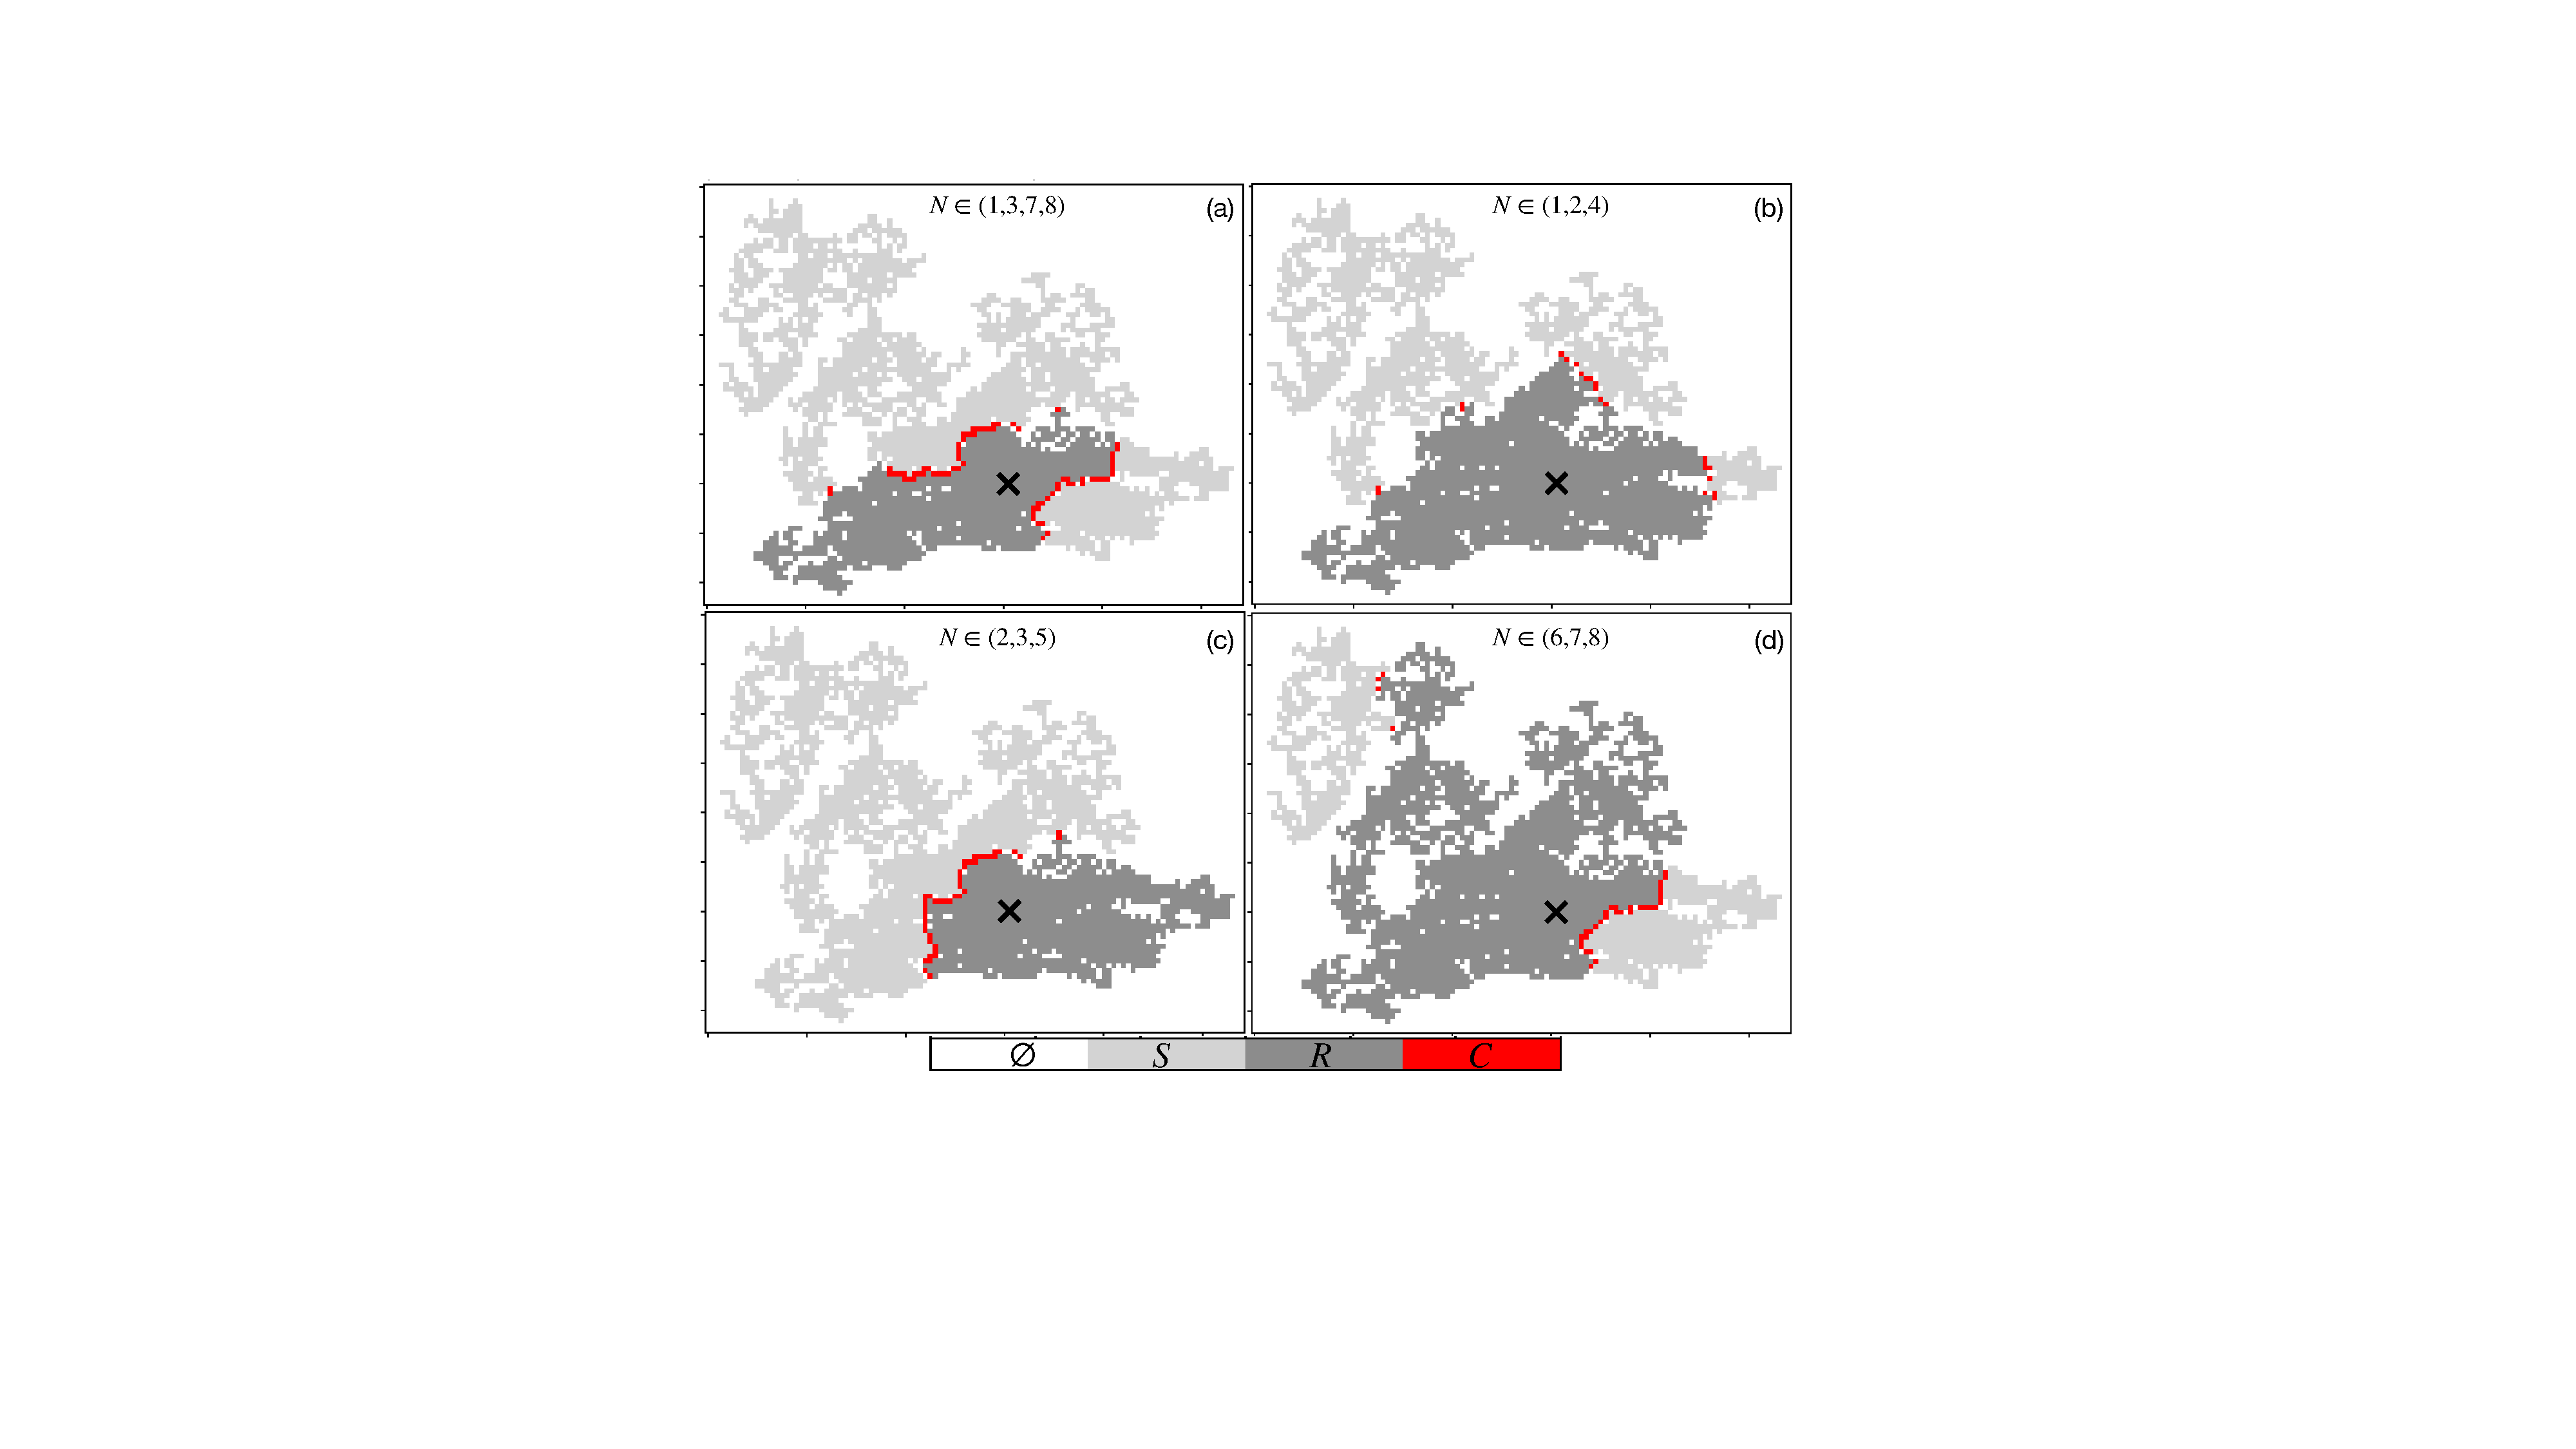
\includegraphics[scale=0.575]{chapter7/figures/figure3-scenario-test.pdf}
    \caption{
    A variety of different control choices are possible for each epicentre, based on the landscape-level host aggregation. 
    Here, the algorithm recursively fragments the target cluster $\mathbf{C}$ through $N=25$ iterations, 
    then different combinations of connecting patches can be used to contain the outbreak in a variety of ways.
    Panels (a-d) represent a small sample of control scenarios for an arbitrary epicentre marked by the central black cross.
    Red patches indicate where landscape-level control $C$ should be targeted to contain the epidemic.
    Light grey patches remain susceptible ($S$) whilst dark grey parches are assumed removed/at-risk, denoted by $R$.
    In practice, every possible control scenario is assessed against every possible epicentre.
     }
    \label{fig:scenario-expo}
\end{figure}

Lastly, it is worthwhile to describe some edge cases and complexities that arise when determining containment scenarios.
Suppose that containment is detected about an epicentre by combining the connecting patches identified in two arbitrary iterations $N_i$ and $N_j$.
In this scenario, some patches from $N_i$ and $N_j$ may be located away from the containing sub-clusters boundary, i.e. in distant (non-bounding) locations.
Thus, irrelevant (non-connecting) patches were identified by employing the binary dilation operator; in this way, only patches neighbouring the confining sub-clusters perimeter contribute to $N_C$.
Moreover, combinations of connecting-patch iterations that failed to define a confining sub-cluster about the epicentre must be ruled out from the analysis.

\newpage

\subsection{Results: control payoff}

Containment scenario payoffs were assessed against all possible epicentres in Great Britain.
For each scenario, the sub-cluster centre of mass (COM) defines an epicentre, i.e. we compute the COM for each sub-cluster produced from $N=20$ iterations of target-cluster fragmentation. 
As before, `target cluster' refers to the largest dominating cluster detected in the $R_0$ map for each $\beta$-valued domain.
Containment scenarios can then be determined for each epicenter\textemdash as described above.
The payoff ratios were then ranked according to the payoff ratio $N_S/ (N_R\times N_C)$, as shown in Figure \ref{fig:payoff-efficiency}\textemdash 
all panels consider the model $\phi_1$-ga resolved to $\mathrm{5 km \times 5 km}$ sized patches.

Figure \ref{fig:payoff-efficiency}(a) presents the top $25$ epidemic containment scenarios over a range of infectiviy parameters in the interval $\beta^* \in [0, 1000]$. 
The reader is referred back to Chapter \ref{ch:6-adb} (i.e. Figures \ref{fig:inverse-power-law-clustering} and \ref{fig:gaussian-clustering-A}) for background information on cluster size with infectiviy $\beta^*$.
Beyond $\beta^*=200$, each value of infectivity involved a large number of containment scenarios, i.e. typically between $10^3-10^4$ containment scenarios per $\beta^*$ parameter.
The payoff ratio starts small with low infectivity values and begins to peak before dropping off. 
The control payoff is low for low values of $\beta^*$ since the number of trees saved is generally lower on account of small susceptible clusters.
Figure \ref{fig:payoff-efficiency}(a) therefore indicates that this strategy of control is not desirable for pathogens with low infectivities.

For exceptionally high values of $\beta^*$, a small number of control scenarios record high-valued payoff ratios, plotted in the shaded region Figure \ref{fig:payoff-efficiency}(a);
this arises on account of efficient edge-location control that saves vast swathes of the host population with a low number of host removals.
Arguably, this represents a limitation of the payoff ratio, as we've defined in this Chapter, because in reality edge-location control is highly idealistic and unlikely to be realised.

Interestingly, Figure \ref{fig:payoff-efficiency}(a) indicates that regional epidemic containment is most efficient over a specific parameter regime,
since the highest payoff scenarios occur in the interval $\beta^* \in [400, 600]$.
Nonetheless, these are preliminary indications. 
As section \ref{sec:gaussian-r0-clustering} demonstrated, nearest-neighbour structuring elements do not scale with changes landscape-level resolution.
Given that Figure \ref{fig:payoff-efficiency}(a) is based on $\phi_1$-ga at the resolution $5\mathrm{km} \times 5\mathrm{km}$, the results presented by Figure \ref{fig:payoff-efficiency}(a)
are likely to change if containment scenarios are computed with smaller patch sizes.
Although Figure \ref{fig:payoff-efficiency}(a) demonstrates an important observation, 
more work is needed to be confident that regional containment is most effective over the interval $\beta^* \in [400, 600]$.

Figure \ref{fig:payoff-efficiency}(b) illustrates the complete set of scenario tests for $\beta^*=500$ (i.e. the $\beta^*$ parameter that registered the highest control payoff).
The number of saved patches that remain in $S$ (i.e, $N_S$) is plotted against $N_R \times N_C$.
The upper and right-hand marginal plots show the corresponding probability density functions for $N_S$ and $N_R \times N_C$.
Each PDF shows a skewed distribution, with most scenarios involving a smaller value of $N_S$ and $N_R \times N_C$.
Of the $3850$ containment scenarios, a small number of high performing tests populate the bottom right-hand quadrant, when $N_S$ is large and $N_R \times N_C$ is low.
This region in the plot represents scenarios where containment is most efficient i.e. the right and left-hand distribution tails when $N_S$ is large and $N_R \times N_C$ is small.

Figures \ref{fig:payoff-efficiency}(c-e) show three scenarios of interest, orange and blue clusters depict removed/at-risk and susceptible/saved patches, respectively. 
Red crosses indicate where the control should be focused to achieve containment. 
Figure \ref{fig:payoff-efficiency}(c), depicts the likely scenario with a central focus of infection.
Most of GB remains at risk, yet some Northern and Southern regions surrounding the target cluster remain protected from the pathogen.
If the disease has not yet reached the connecting patches (identified by the red crosses), Figure \ref{fig:payoff-efficiency}(c) indicates that regional containment might be attempted alongside targeting a disease wave-front \cite{large-scale-control}, or more local-scale pathogen eradication \cite{WEBIDEMICS}. 
Although, ultimately, more work is needed to assess the efficacy and possibility of halting/slowing the spread.

\begin{figure}
    \centering
    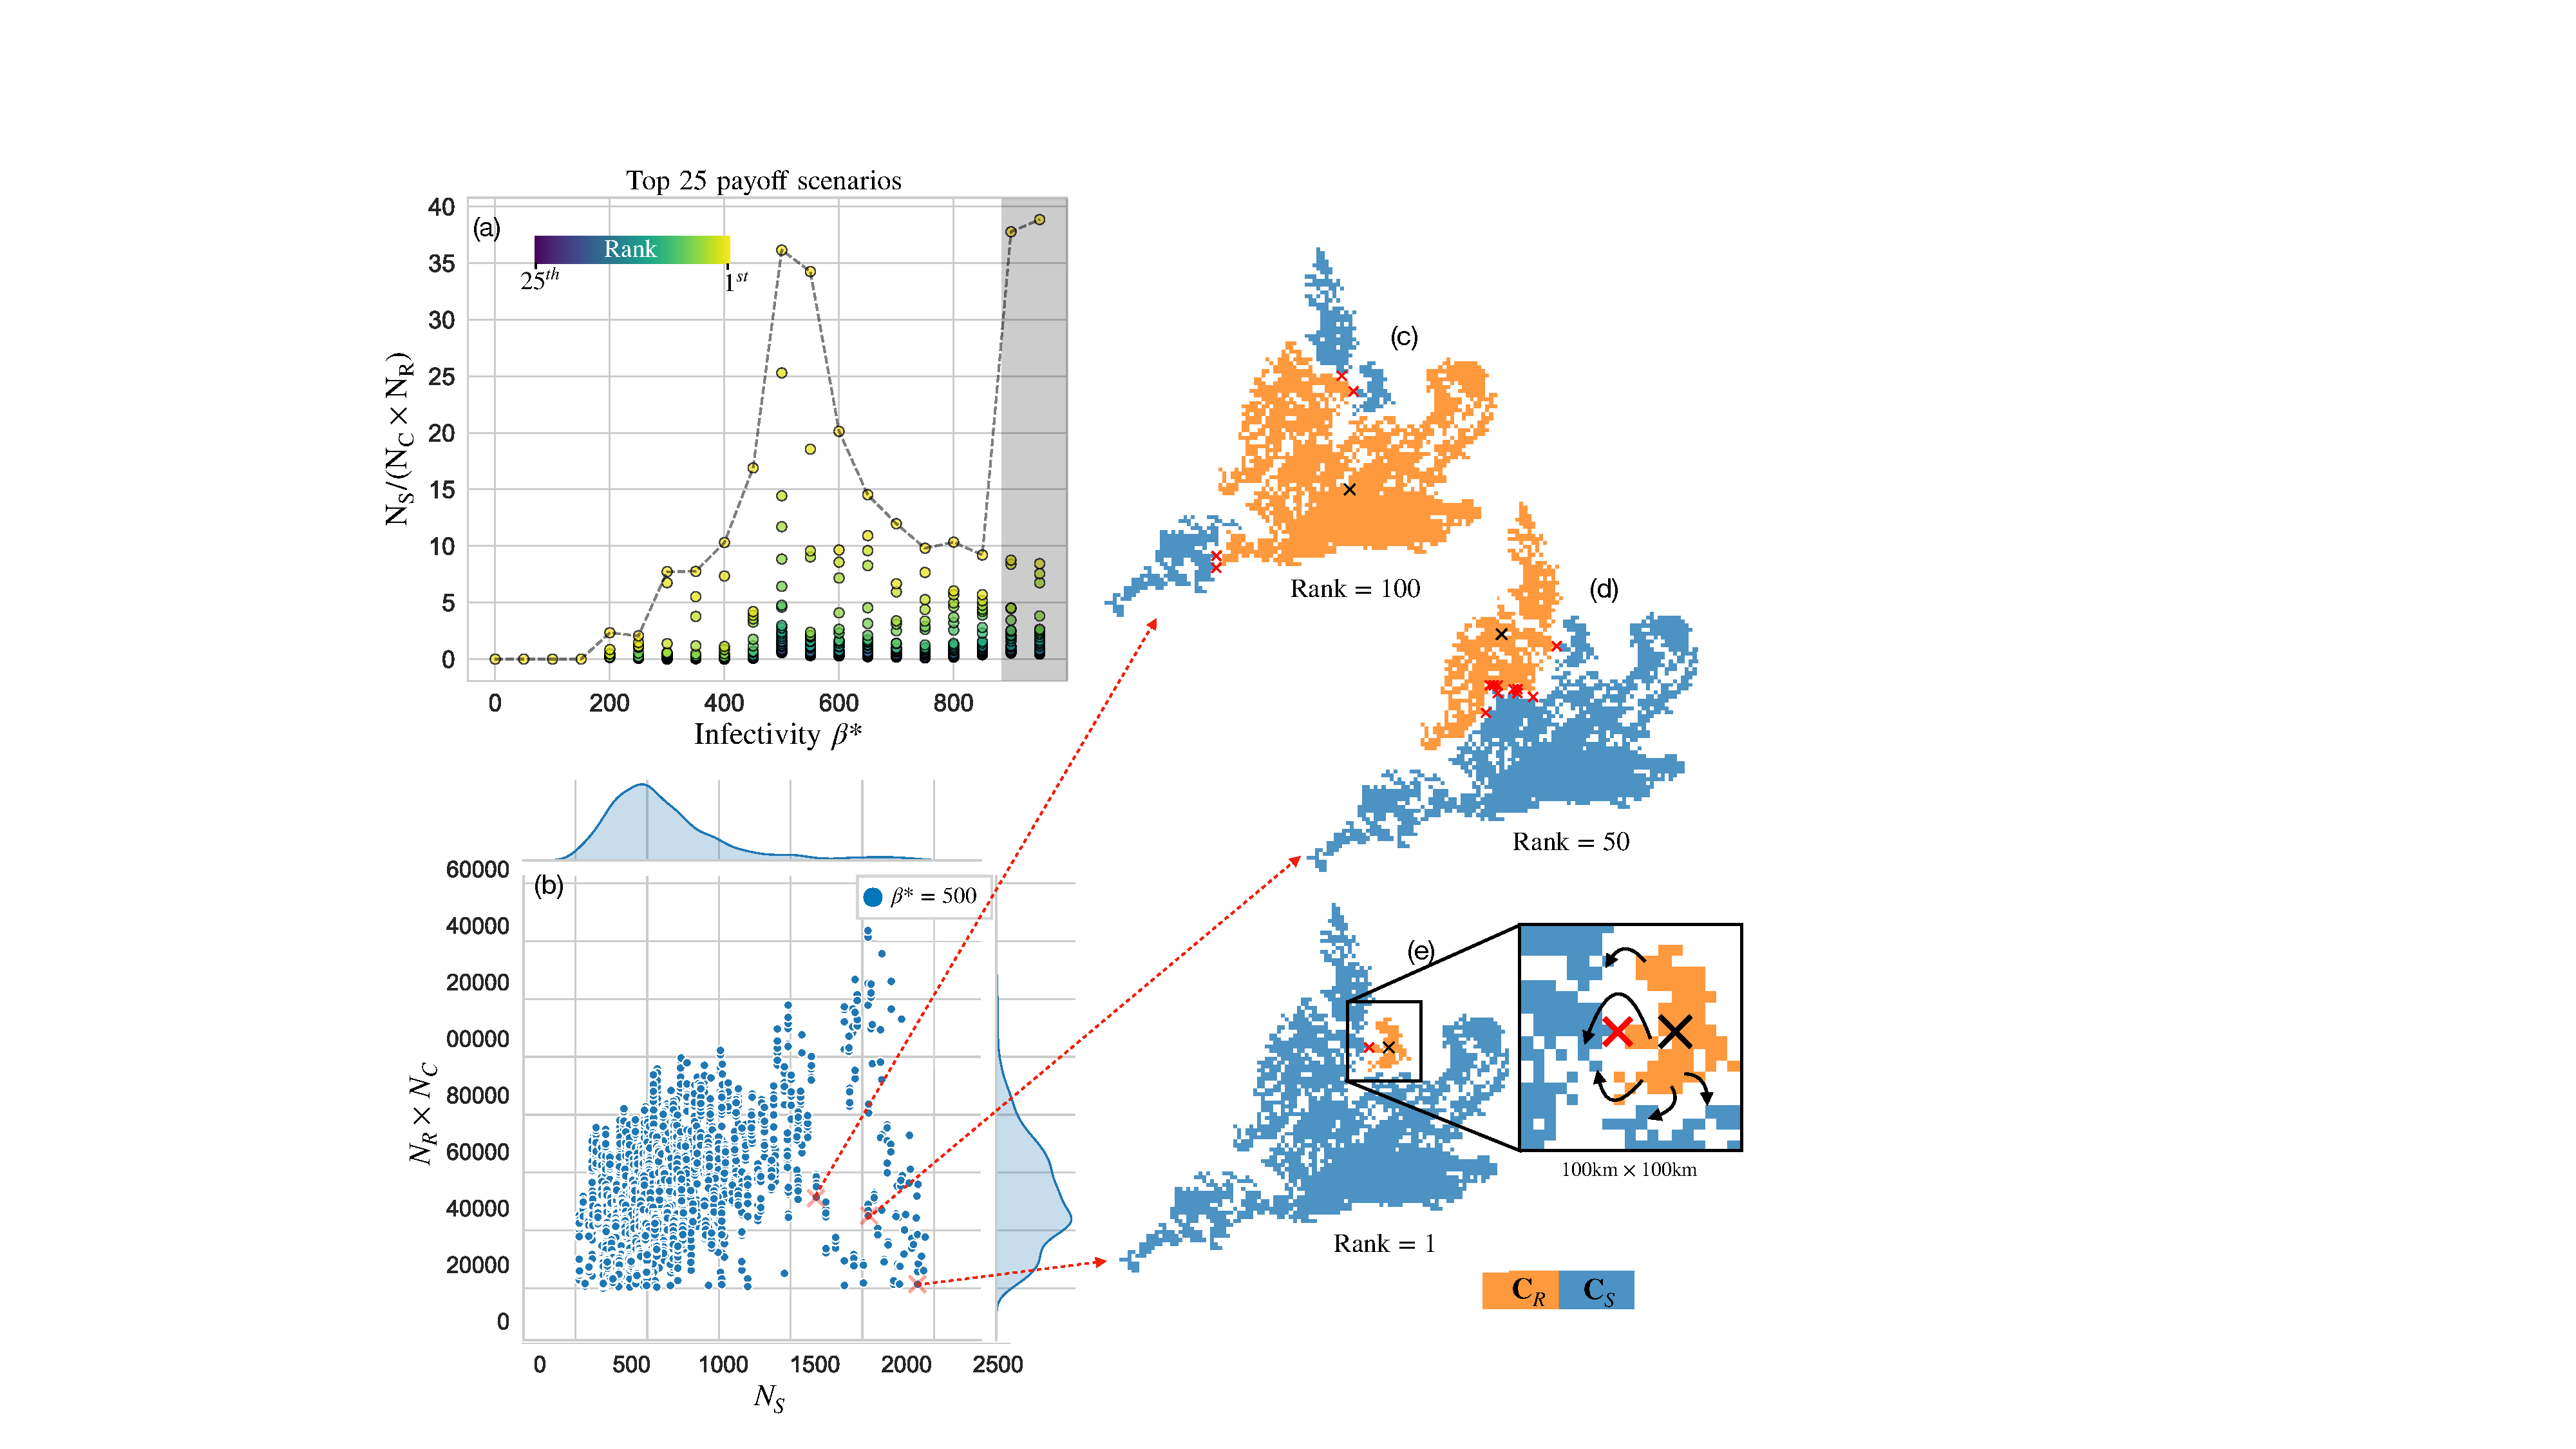
\includegraphics[scale=0.45]{chapter7/figures/figure4-scenario-payoff.pdf}
    \caption{The control `payoff' is accessed by comparing the number of patches that remain susceptible ($N_S$) against the number of patches removed ($N_R$) and controlled ($N_C$).
             (a) The payoff ratio $N_S / (N_R \times N_C)$ is plotted against the infectiviy parameter $\beta^*$ for the top $25$ highest payoff scenarios.
             (b) The complete list of (3850) different scenario tests are plotted for the highest payoff infectivity parameter $\beta^*=500$; the lower right-hand quadrant defines the most efficient control scenarios.
             (c-e) Spatial plots that show three hypothetical scenarios from panel (b), with payoffs ranked 1, 50, 100. 
             Blue and orange clusters outline patches that remain susceptible and become removed, respectively.
             }
    \label{fig:payoff-efficiency}
\end{figure}

The targeted control patches in Figure \ref{fig:payoff-efficiency}(d) resemble those identified previously in Figure \ref{fig:R0-threshold-function}(e), yet this time for a higher $\beta^*$-valued domain at a lower landscape-level resolution.
Desirably, observing connecting patches in approximately the same location for different infectivity values suggests that some patches may be important for control at various epidemic scales.
Moreover, Figure \ref{fig:payoff-efficiency}(d) hints toward there being similarities at and different resolutions\textemdash the concern mentioned above.

Figure \ref{fig:payoff-efficiency}(e) reveals the highest payoff result for $\beta^*=500$.
In this scenario, the epicentre lies close to the Eastern coastline (Skegness), 
and the control area is located slightly inland (approximately between Lincoln and Sheffield).
The zoomed inset highlights a single $\mathrm{5km \times 5 km}$ patch, and control saves the vast majority of GB from infection.
This scenario is no doubt idealistic and unlikely to be realised in a real-life outbreak.
In a real-life outbreak, epicentres are unlikely to be so conveniently located about the coastline.
Furthermore, detecting and controlling the pathogen remains difficult before it spreads to distant (and more centralised) locations.
Nevertheless, Figure \ref{fig:payoff-efficiency}(e) reinforces the intuitive notion that epicentres around edge positions are contained efficiently.
The inset highlights where pathogen dispersal might jump between clusters, indicated by the curved arrows.
Although wind-dispersed secondary infections are likely rare over these spatial scales ($5$-$20\mathrm{km}$), they are nevertheless thought possible for fungal spores \cite{grosdidier2018tracking};
the analysis presented here neglect these complexities, which requires further investigation.

% The last spatial plot, Figure \ref{fig:payoff-efficiency}(c), depicts a more likely scenario with a centrally located focus.
% Most of GB remains at risk, yet some Northern and Southern regions surrounding the target cluster remain protected from the pathogen.
% If the disease has not yet reached the connecting patches (identified by the red crosses), Figure \ref{fig:payoff-efficiency}(c) indicates that regional containment might be attempted alongside targeting a disease wave-front \cite{large-scale-control}, or more local-scale pathogen eradication \cite{WEBIDEMICS}. 
% Although, ultimately, more work is needed to assess the efficacy and possibility of halting/slowing the spread.

\newpage 

\section{Discussion and future research}

This Chapter outlined a conceptual strategy of landscape-level control, targeting a pathogens local wind-dispersal mechanism.
The strategy aims to preferentially control the pathogen through identified patches in the host population. 
In an idealistic scenario, cluster fragmentation can be achieved along with `regional containment' if the identified patches are taken below the epidemic threshold.
Nonetheless, fungal spores are thought to be able to disperse over large distances, e.g. from mainland Europe to Great Britain \cite{wylder2018evidence, freer2017tree}.
Given that the effects of LDD (beyond $5\mathrm{km}$) were neglected, the utility, efficiency and practicality of real-life implementation remain unproven. However, the work undertaken in this Chapter sets the scene for future investigations.

Various large-scale models have examined spread over contiguous cells, or patches, e.g. \cite{gaydos2019forecasting, large-scale-control, meentemeyer2011epidemiological}.
However, to our knowledge no large-scale studies involve the spatial arguments based on population heterogeneity presented in this Chapter.
Although the idea of density reductions unpinned control in this work (consistent with more traditional methods of eradication),
the possibility of other biological control methods remains an attractive option, e.g. fungicide treatments \cite{hauptman2015application}.

Targeted epidemic control goes hand-in-hand with an on-the-ground understanding of which regions become infected.
Subsequently, the method presented to identify high-risk areas might find applications in enhanced monitoring and surveillance \cite{surveillance-review}, discussed previously in section \ref{sec:modelling-and-policy}. Consequently, future work could access the method of critical/connecting patch detection for enhanced landscape-level monitoring.

The algorithm constructed in section \ref{sec:fragmentation-method} presented a means to identify `connecting patches', which if taken below $R_0=1$ would fragment the cluster.
Related concepts of network fragmentation exist in telecommunications \cite{albert2000error}, ecological space modeling \cite{luo2021understanding} and human epidemiology \cite{chami2017social}.
However, no sources could be found relating to spatially-explicit epidemic spread over a landscape of trees.
The algorithm described in \ref{sec:fragmentation-method} treated patches below the threshold as negligible, without this assumption CCA would cease to work.
Given the possibility of stochastic below-threshold spread, future work should move towards a generalised (risk-based) scheme that factors in the presence of patches below $R_0=1$;
in such a scheme, we may ultimately question the choice of CCA due to its binary nature and inability to describe non-local coupling. Subsequently, routes to progress and improve the framework and control strategy are outlined below.

% Nevertheless, the results of section \ref{sec:cast-study-jump-patches} provide indications that pathogen dispersal might, at worst, be slowed by performing patch-level density reductions;
% in the best-case scenario, policymakers and forest managers might gain vital time to respond to the threat of invasion and tree populations provided with crucial recovery time.

% The chapter begins by investigating the probability of patch-to-patch transmission with distance.
% Then, using the $SEIR$ model of ADB, we access the probability of invasion as a function of the distance between patches\textemdash
% a facet overlooked by the nearest-neighbour based $R_0$-maps presented previously.
% Then, considering a coupled system of three patches, section \ref{sec:density-reductions} examines intermediary-patch density reductions for epidemic control.


% - \cite{mcleish2021structuring} <-- discuss 

% The article published by \cite{time-varying-infectivity} indicates the possibility of \textit{preferentially} controlling an area based on the final-sized epidemic. 
% However, we outline the possibility it might be more beneficial to preferentially control an area based on its spatial location and how it couples to to neighbouring areas.

% LDD
% pathogen dispersal depends on a myriad of factors, size, aerodynamics, production-quantity, and life-times to name a few.
% rod-like bacterium less, aerodynamic, and subject to a more localised dispersal kernel? As such, the method outlined in this chapter could be better suited... 

% Genetic tolerance
% - genetic tolerance is currently the only viable strategy of control\cite{kosawang2018fungal}

\begin{figure}
    \centering
    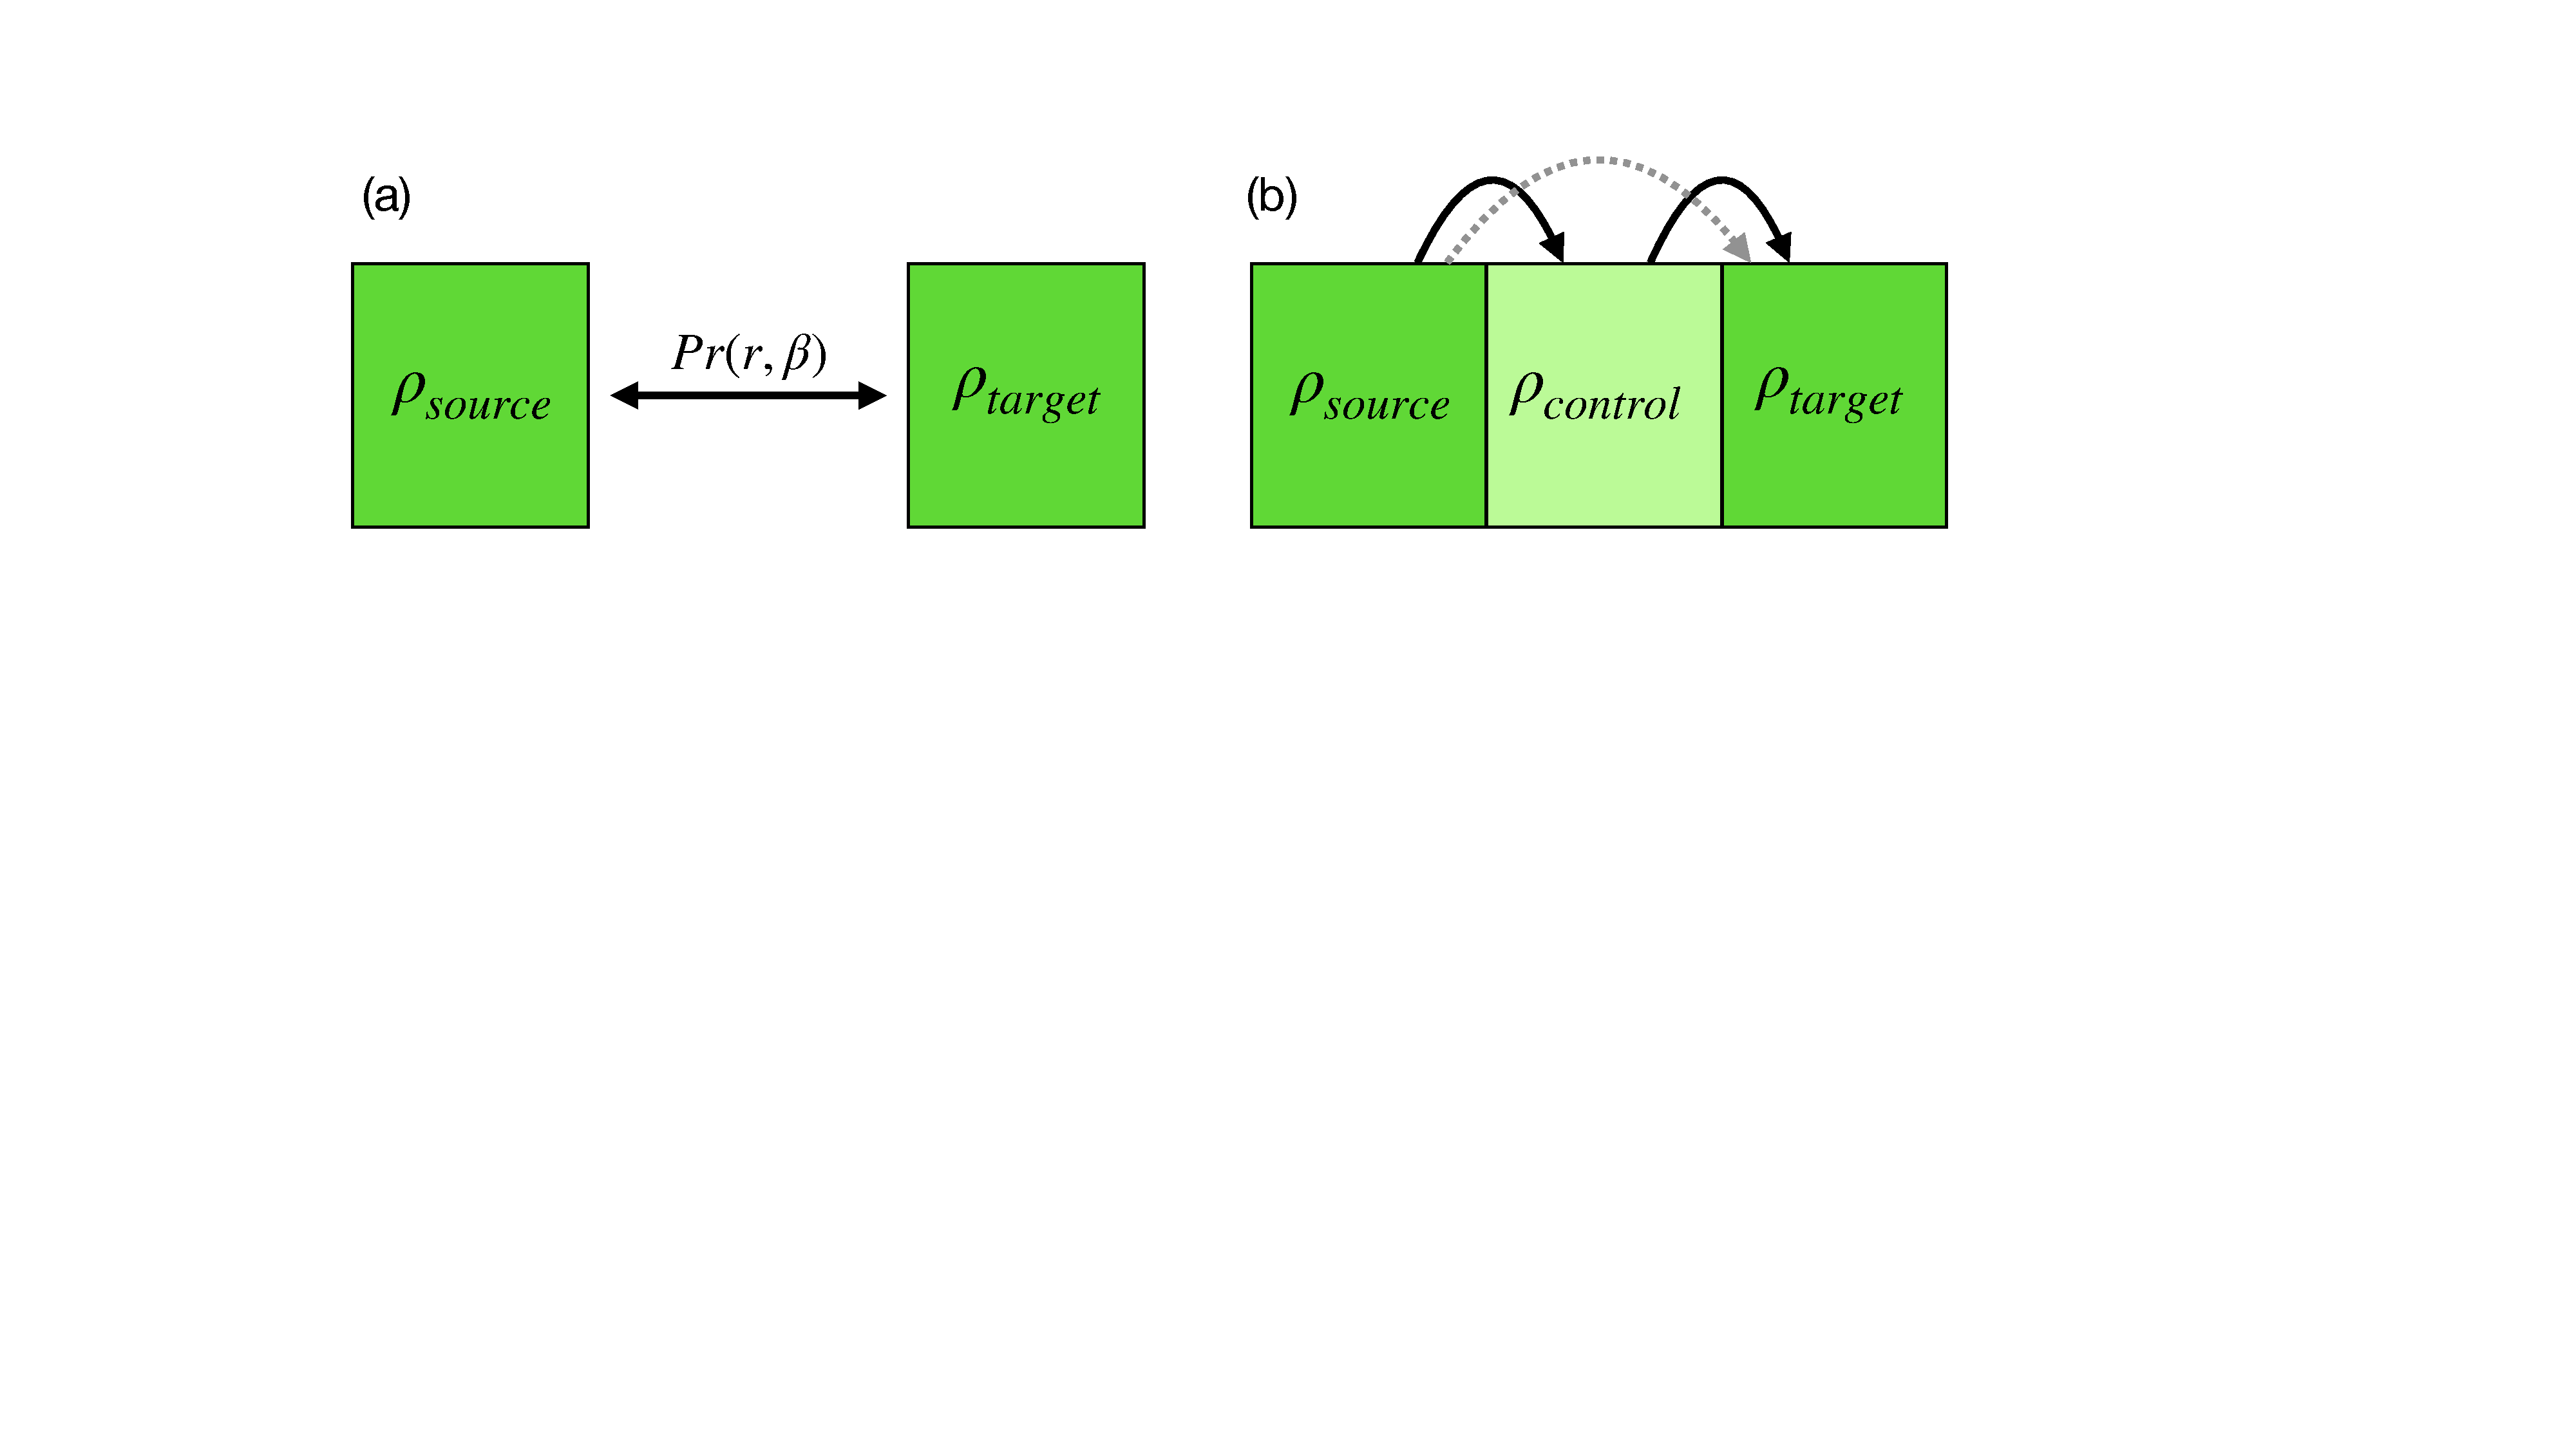
\includegraphics[scale=0.35]{chapter7/figures/figure5-future-reserach.pdf}
    \caption{A diagram illustrating potential research avenues to improve framework and better evaulate the control strategy. 
    (a) Examining the transmission probability between a source and target patch as a function of distance $r$ and infectivity $\beta$. 
    (b) Understanding the degree to which control of an intermediary patch ($\rho_{control}$) can disrupt dispersal between a source and target patch.}
    \label{fig:future-research}
\end{figure}

\subsection{Future research questions}
\label{sec:future-questions}
Throughout Chapters \ref{ch:6-adb} and \ref{ch7:landscape-level-control}, nearest-neighbour connectivity underpinned $R_0$-map clustering.
Ultimately, this followed from defining $R_0$-maps based solely on `within-patch' interactions. Moving forward, we require an enhanced understanding of `between-patch' interactions.
Figure \ref{fig:future-research} illustrates two future research questions that could help develop the framework and assess the utility of landscape-level control.

\subsubsection{Patch-to-patch transmission}
A modelling setup could define two patches, a source patch ($\rho_{source}$) that hosts the infection at $t=0$, and an infection-free target patch ($\rho_{target}$). Ideally, patches should mirror the highest possible resolution\textemdash given by $1\mathrm{km^2}$ for the maps of predicted ash abundance given by \cite{hill.data}.
One could then assess the transmission probability between $\rho_{source}$ and $\rho_{target}$ as a function of distance $r$ and infectivity $\beta$, reflected in Figure \ref{fig:future-research}(a). 
A similar on-the-ground experiment was conducted by \cite{https://doi.org/10.1111/1365-2745.13383},
who accessed the prevalence of collar canker and rachis symptoms in neighbouring ash. 
The authors found that the influence of ADB decayed exponentially up to $200-300\mathrm{m}$ away from a high-density source.

Although inverse power laws are more likely to describe the spread of ADB, contrasting the transmission probability between Gaussian and power-law dispersal models for different levels of $\beta$ could prove insightful. In particular, this examination could provide two length-scales, above which transmission patch-to-patch is unlikely.  Such insights could help understand the disease spread between infected ash stands and help bolster the knowledge of forest managers, especially when constructing new stands.

If the source patch reflects on-the-ground observations of infected areas, we can speculate about constructing a `transmission probability' map in GB. In theory, an ensemble average calculating the transmission probability as a function of distance $r$, infectivity $\beta$ and target/source densities could be projected onto the map of predicted ash abundance.
Then, we could aim to construct a probability map depicting which neighbouring regions are likely to become infected. An accurate and reliable probability map could provide immense value to rapid-response control initiatives by helping direct the allocation of resources in the early phases of an invasion. 
Although, this notion undoubtedly requires effective monitoring and surveillance to detect disease inside infected patches before the disease has had time to propagate over large areas.

\subsubsection{Between-patch control}

Lastly, targeted control rests on artificially reducing $R_0$ below unity\textemdash outlined in section \ref{sec:towards-regional-control}.
Subsequently, non-existent epidemic spread was assumed for patches $R_0=1$.
More research is required to understand this assumption and further assess the efficiency of control.
In addition, resource constraints were neglected. In reality, control initiatives are limited by governmental budgets and the funding made available to stakeholders.
Therefore, any robust control strategy should make efforts to incorporate the influence of government budgets in large-scale control \cite{large-scale-control}.

Figure \ref{fig:future-research}(b) illustrates a potential setup to progress the understanding of landscape-level control by considering a system of three coupled patches.
The coupled system shown in Figure \ref{fig:future-research}(b) is similar to Figure \ref{fig:future-research}(a), although this time an intermediary `control' patch separates the target and source patches. In this system, dispersal can either jump between or directly over the control patch, shown by the solid black and dashed grey arrows, respectively. In $\rho_{control}$, control can be achieved by reducing tree density through sanitation felling or by reducing $\beta$ (mirroring biological control, e.g. fungicide treatments).

Studying the effect of different control measures in $\rho_{control}$ could provide crucial insight into the control strategy proposed in this Chapter.
In particular, by studying the number of infected trees that arise in $\rho_{target}$ conditional on different control measures. 
Intuitively, we could expect efficient control when propagation occurs through a thin-tailed Gaussian kernel.
However, for fat-tailed dispersal kernels, the efficacy of between-patch control remains far less obvious and subject to more scrutiny.
In summary, three hypothetical outcomes can be expected from studying the coupled system: 
\begin{enumerate}
    \item Between-patch control is insufficient because large numbers of secondary infections arise in $\rho_{target}$ due to infected trees in $\rho_{source}$.
    \item The development of an outbreak in $\rho_{target}$ is slowed down by control measures in $\rho_{control}$, albeit conditioned on the epidemic and control parameters.
    \item Complete epidemic containment between patches can be achieved, thereby preventing the pathogen from propagating to $\rho_{target}$.
\end{enumerate}
For inverse power law dispersal, complete epidemic containment, as described in (3), is unlikely due to its fat-tail.
However, future research could assess the degree to which control slows down the spread between patches, conditioned on epidemic and control parameters. Although, the answer to these questions remains open to investigation.

\newpage












